\section*{Introduction}

MiniFrame is a C library providing a framework to implement the MiniMax algorithm.\\ 

The user can define the system to which the MiniMax algorithm is apply by implementing the set of functions in files \begin{ttfamily}miniframe-model.h\end{ttfamily}, \begin{ttfamily}miniframe-inline-model.c\end{ttfamily} and \begin{ttfamily}miniframe-model.c\end{ttfamily}.\\

It supports one or several actor(s) and uses a time limit to control MiniMax expansion. MiniFrame uses time prediction to maximise the number of steps computed inside the time limit and minimize the risk of overcoming this time limit.\\

The user can choose if MiniFrame should try to reuse previously computed worlds or recompute several times the same world if it's reachable through several transitions. If it reuses previously computed worlds MiniFrame provide the percentage of reused worlds at each step. MiniFrame also provide the time unused and the number of computed worlds at each step to allow the user to estimate performances.\\

A basic example is given to illustrate how to use MiniFrame, as well as the implementation for the game of Oware.\\

The example of the game of Oware also contains an implementation of how to combine MiniFrame with ELORank, GenAlg and NeuraNet to train a NeuraNet later used as the evaluation function of the MiniFrame.\\

It uses the \begin{ttfamily}PBErr\end{ttfamily}, \begin{ttfamily}PBMath\end{ttfamily} and \begin{ttfamily}GSet\end{ttfamily} libraries.\\

\section{Interface}

\subsection{miniframe.h}

\begin{scriptsize}
\begin{ttfamily}
\verbatiminput{/home/bayashi/GitHub/MiniFrame/miniframe.h}
\end{ttfamily}
\end{scriptsize}

\section{Code}

\subsection{miniframe.c}

\begin{scriptsize}
\begin{ttfamily}
\verbatiminput{/home/bayashi/GitHub/MiniFrame/miniframe.c}
\end{ttfamily}
\end{scriptsize}

\subsection{miniframe-inline.c}

\begin{scriptsize}
\begin{ttfamily}
\verbatiminput{/home/bayashi/GitHub/MiniFrame/miniframe-inline.c}
\end{ttfamily}
\end{scriptsize}

\section{Makefile}

\begin{scriptsize}
\begin{ttfamily}
\verbatiminput{/home/bayashi/GitHub/MiniFrame/Makefile}
\end{ttfamily}
\end{scriptsize}

\section{Unit tests}

\begin{scriptsize}
\begin{ttfamily}
\verbatiminput{/home/bayashi/GitHub/MiniFrame/main.c}
\end{ttfamily}
\end{scriptsize}

\section{Unit tests output}

\begin{scriptsize}
\begin{ttfamily}
\verbatiminput{/home/bayashi/GitHub/MiniFrame/unitTestRef.txt}
\end{ttfamily}
\end{scriptsize}

\section{Examples}

\subsection{Basic example}

\subsubsection{miniframe-model.h}

\begin{scriptsize}
\begin{ttfamily}
\verbatiminput{/home/bayashi/GitHub/MiniFrame/Examples/BasicExample/miniframe-model.h}
\end{ttfamily}
\end{scriptsize}

\subsubsection{miniframe-model.c}

\begin{scriptsize}
\begin{ttfamily}
\verbatiminput{/home/bayashi/GitHub/MiniFrame/Examples/BasicExample/miniframe-model.c}
\end{ttfamily}
\end{scriptsize}

\subsubsection{miniframe-inline-model.c}

\begin{scriptsize}
\begin{ttfamily}
\verbatiminput{/home/bayashi/GitHub/MiniFrame/Examples/BasicExample/miniframe-inline-model.c}
\end{ttfamily}
\end{scriptsize}

\subsection{Oware}

\subsubsection{miniframe-model.h}

\begin{scriptsize}
\begin{ttfamily}
\verbatiminput{/home/bayashi/GitHub/MiniFrame/Examples/Oware/miniframe-model.h}
\end{ttfamily}
\end{scriptsize}

\subsubsection{miniframe-model.c}

\begin{scriptsize}
\begin{ttfamily}
\verbatiminput{/home/bayashi/GitHub/MiniFrame/Examples/Oware/miniframe-model.c}
\end{ttfamily}
\end{scriptsize}

\subsubsection{miniframe-inline-model.c}

\begin{scriptsize}
\begin{ttfamily}
\verbatiminput{/home/bayashi/GitHub/MiniFrame/Examples/Oware/miniframe-inline-model.c}
\end{ttfamily}
\end{scriptsize}

\subsubsection{main.c}

\begin{scriptsize}
\begin{ttfamily}
\verbatiminput{/home/bayashi/GitHub/MiniFrame/Examples/Oware/main.c}
\end{ttfamily}
\end{scriptsize}

\subsubsection{Makefile}

\begin{scriptsize}
\begin{ttfamily}
\verbatiminput{/home/bayashi/GitHub/MiniFrame/Examples/Oware/Makefile}
\end{ttfamily}
\end{scriptsize}

\subsubsection{Example}

exampleGame.txt:\\
\begin{scriptsize}
\begin{ttfamily}
\verbatiminput{/home/bayashi/GitHub/MiniFrame/Examples/Oware/exampleGame.txt}
\end{ttfamily}
\end{scriptsize}

training.txt:\\
\begin{scriptsize}
\begin{ttfamily}
\verbatiminput{/home/bayashi/GitHub/MiniFrame/Examples/Oware/training.txt}
\end{ttfamily}
\end{scriptsize}

ELO rank of the best NeuraNet (blue) as evaluation function and ELO rank of the standard (red) evaluation function, and rank of the standard evaluation function against a pool of 21 NeuraNet:\\

\begin{center}
\begin{figure}[H]
\centering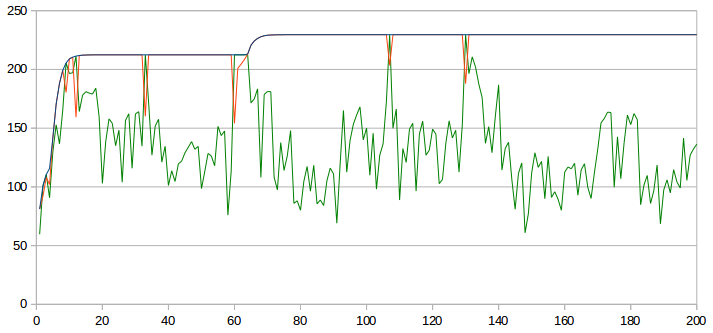
\includegraphics[width=10cm]{/home/bayashi/GitHub/MiniFrame/Examples/Oware/training.png}\\
\end{figure}
\end{center}
